\subsection{Experiment details}
\label{subsec:app_exp_detail}
\begin{table}
	\caption{The configuration for Gaussian kernel and the search grid for initial learning rate on the Census, YearPred, Covtype and TIMIT datasets.}
	\label{tab:hyperparam}
	\begin{center}
	\begin{tabular}{lll}
	\toprule
	Dataset & $1/2\sigma^2$ & Learning rate grid \\
	\midrule
Census & 0.0006 & {0.01, 0.05, 0.1, \textbf{0.5}, 1.0} \\
YearPred & 0.01 & {0.05, 0.1, \textbf{0.5}, 1.0, 5.0} \\
Covtype & 0.6 & {1.0, 5.0, 10.0, \textbf{50.0}, 100.0} \\
TIMIT & 0.0015 & {5.0, 10.0, 50.0, \textbf{100.0}, 500.0} \\
	\bottomrule
	\end{tabular}
	\end{center}
	\label{tab:kernel_hyper}
\end{table}

\paragraph{Dataset details and kernel configuration}
In section~\ref{sec:experiments}, we demonstrate the performance of LP-RFFs on the TIMIT, YearPred, CovType and Census datasets, with SGD-based minibatch training. These datasets spans over regression, binary and multi-class classification tasks. We present the details, including task specification, dataset size and the number of raw data attributes in Table~\ref{tab:dataset_details}. In these experiments we use Gaussian kernel with the kernel width hyperparameter $\sigma$ recommended by~\cite{may2017} in Table~\ref{tab:kernel_hyper}. 
\begin{table}
	\caption{Dataset details.  For classification tasks, we write the number
		of classes in parentheses in the ``task'' column.}
	\label{tab:datasets}
%	\small
	\begin{center}
		\begin{tabular}{llllll} 
			\toprule
			\textbf{Dataset}  & \textbf{Task} & \textbf{Train} & \textbf{Heldout} & \textbf{Test} & \textbf{\#Attr.} \\ 
			\midrule
			CENSUS   & Reg.   & 16k   & 2k      & 2k   & 119 \\ 
			YEARPRED & Reg.   & 417k  & 46k     & 52k  & 90  \\ 
			COVTYPE  & Class. (2) & 418k  & 46k     & 116k & 54  \\ 
			TIMIT    & Class. (147) & 2.3M  & 245k    & 116k & 440 \\
			\bottomrule
		\end{tabular}
	\end{center}
	\label{tab:dataset_details}
\end{table}

\paragraph{Hyperparameter tuning for SGD-based training}
We use the heldout set in order to perform early stopping and determine when to decay the learning rate, as in \citep{morgan1990generalization,sainath2013b,sainath2013low}. Early stopping can be seen as a form of regularization \citep{zhang2005boosting,wei2017early}, and this saves us the effort of manually tuning the initial learning rate, the learning rate decay, the regularizer, and the number of training epochs.  The scheme works as follows: at the end of each epoch, we decay the learning rate in half if the heldout performance is less than $1\%$ better relative to the previous best model, using MSE for regression and cross entropy for classification. Furthermore, if the model performs \textit{worse} than the previous best, we revert the model. The training terminates after the learning rate has been decayed 10 times. Early stopping can be seen as a form of regularization \citep{zhang2005boosting,wei2017early}.  We use a single initial learning rate per dataset across all experiments, which we tune via grid search using $20\text{k}$ \Nystrom features. We choose to use \Nystrom features to tune the initial learning rate in order to avoid biasing the results in favor of RFF-based approaches.

\paragraph{Hyperparameter tuning for LM-HALP-based training}
We use the same learning rate schedule as the one in the SGD-based experiments. We sweep the $\mu$ parameter, which determines the value of the quantization scale in HALP, using grid search over $\{0.001, 0.01, 0.1, 1.0\}$. For each number of LP-RFFs $m$, we choose the value of $\mu$ attaining lowest heldout classification error, and report this as the error.

\subsection{Additional experiment results}
\label{subsec:app_additional_exp_res}
In Section~\ref{sec:full_run}, we demonstrate the generalization performance of LP-RFFs on the TIMIT and YearPred datasets. In this section, we demonstrate the full generalization performance comparison on the TIMIT, YearPred, CovType and Census datasets. In Figure~\ref{fig:generalization_col_app}, we show the generalization performance of 8, 4, 1 bit LP-RFFs, with FP-\Nystrom, FP-RFF and circulant FP-RFF as the full precision baselines. We can observe that LP-RFF, by using 4 or 8-bit quantized representation, can systematically outperform full precision baselines across the four datasets under different memory budgets.
%\begin{figure}
%	\centering
%	\begin{tabular}{@{\hskip 0in}c@{\hskip 0in}c@{\hskip 0in}c@{\hskip 0in}c@{\hskip 0in}}
%%		\subfigure[Census heldout MSE]{\label{fig:census_mem} 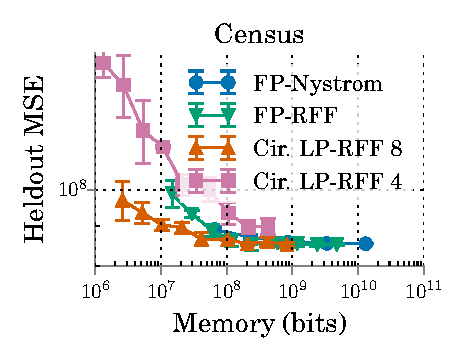
\includegraphics[width=0.3\linewidth]{figures/census_MSE_vs_n_memory.pdf} } \hfill
%%		\subfigure[Census heldout MSE]{\label{fig:census_feat}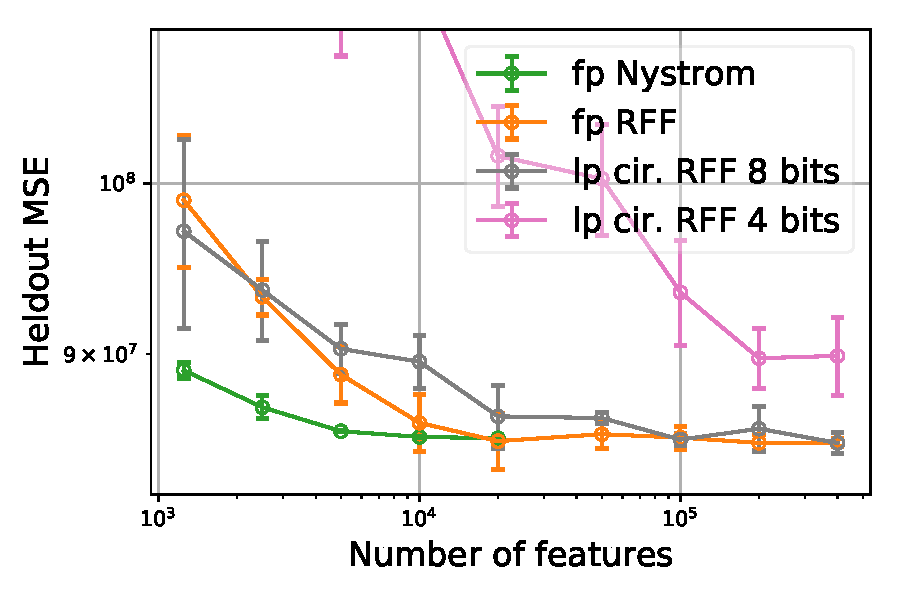
\includegraphics[width=0.3\linewidth]{figures/census_MSE_vs_n_feat.pdf} } \hfill
%%		\subfigure[CovType heldout error]{\label{fig:covtype_mem} 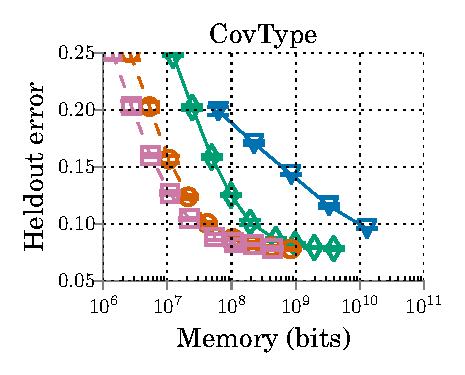
\includegraphics[width=0.3\linewidth]{figures/covtype_error_vs_n_memory.pdf} } \hfill
%%		\subfigure[CovType heldout error]{\label{fig:covtype_feat}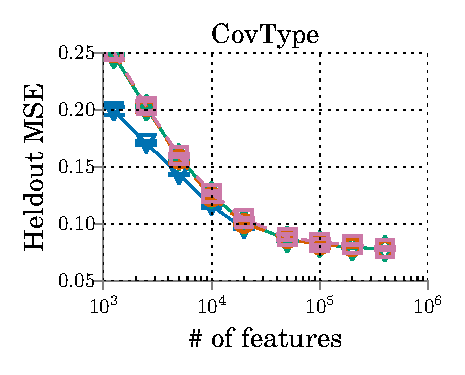
\includegraphics[width=0.3\linewidth]{figures/covtype_error_vs_n_feat.pdf} } \hfill
%%		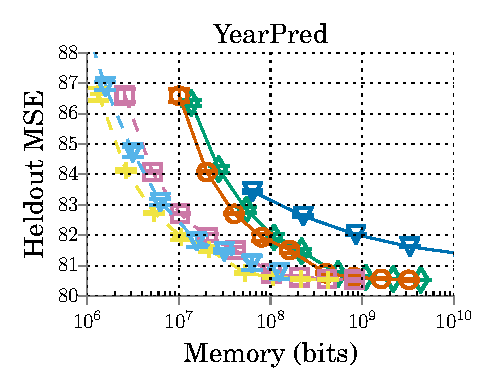
\includegraphics[width=0.3\linewidth]{figures/yearpred_MSE_vs_n_memory_all_line.pdf} &
%%		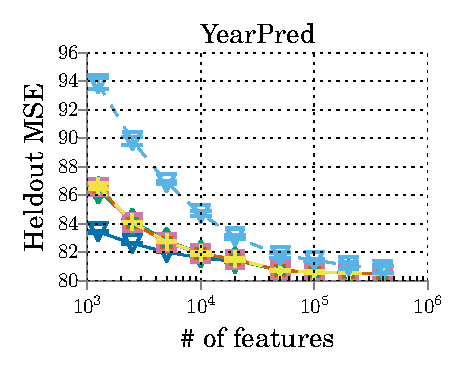
\includegraphics[width=0.3\linewidth]{figures/yearpred_MSE_vs_n_feat_all_line.pdf} &
%%		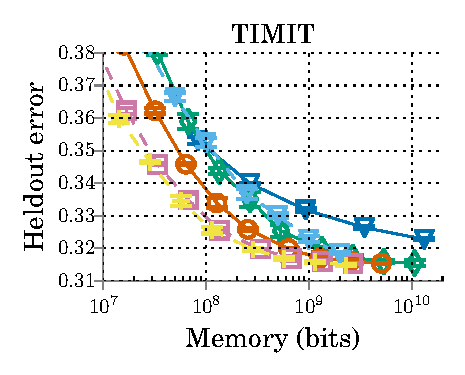
\includegraphics[width=0.3\linewidth]{figures/timit_error_vs_n_memory_all_line.pdf} &
%%		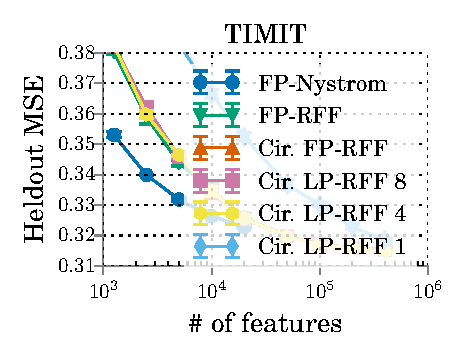
\includegraphics[width=0.3\linewidth]{figures/timit_error_vs_n_feat_all_line.pdf} \\
%%		(a) Census & (b) YearPred & (c) Covtype & (d) TIMIT \\
%		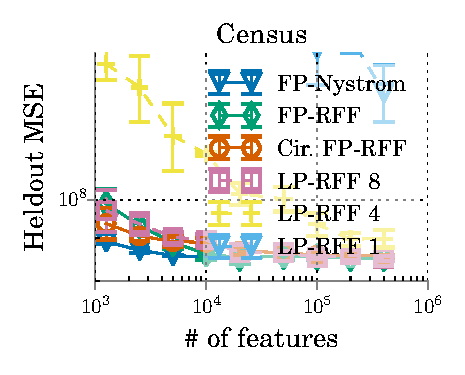
\includegraphics[width=0.26\linewidth]{figures/census_MSE_vs_n_feat_all_line.pdf} &
%		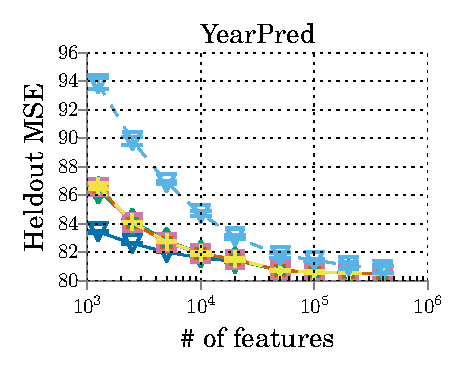
\includegraphics[width=0.26\linewidth]{figures/yearpred_MSE_vs_n_feat_all_line.pdf} &
%		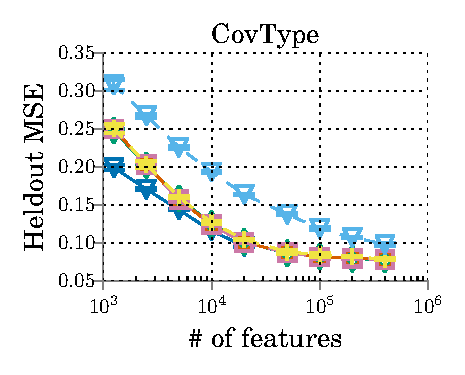
\includegraphics[width=0.26\linewidth]{figures/covtype_error_vs_n_feat_all_line.pdf} &
%		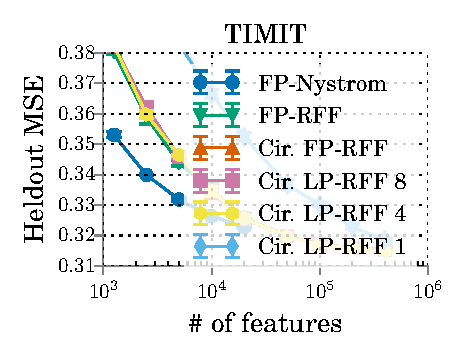
\includegraphics[width=0.26\linewidth]{figures/timit_error_vs_n_feat_all_line.pdf} \\
%		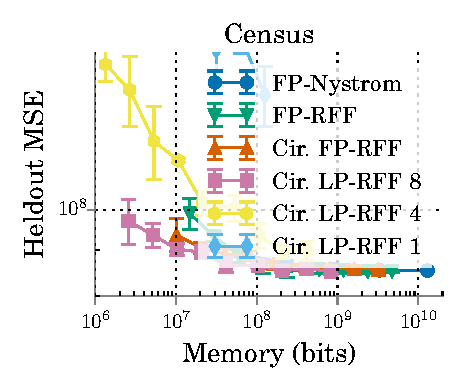
\includegraphics[width=0.26\linewidth]{figures/census_MSE_vs_n_memory_all_line.pdf} &
%		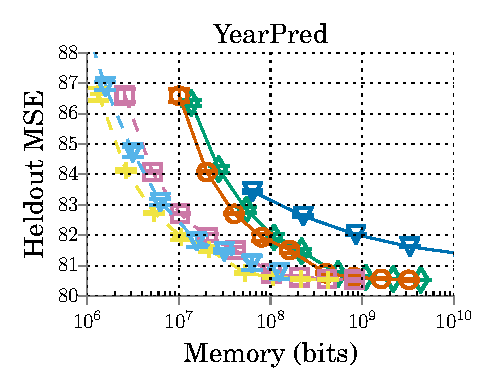
\includegraphics[width=0.26\linewidth]{figures/yearpred_MSE_vs_n_memory_all_line.pdf} &
%		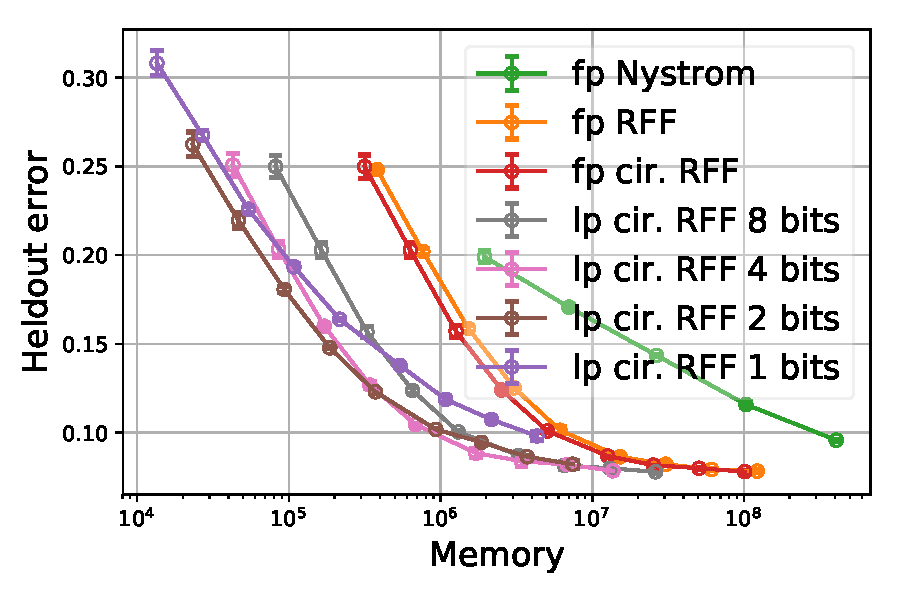
\includegraphics[width=0.26\linewidth]{figures/covtype_error_vs_n_memory_all_line.pdf} &
%		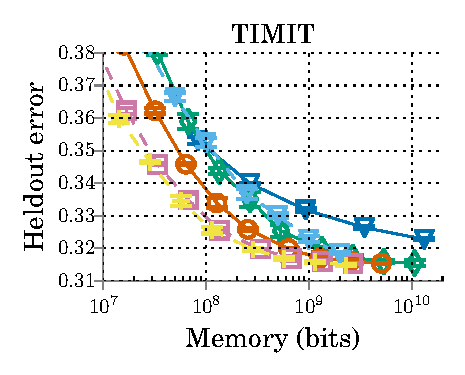
\includegraphics[width=0.26\linewidth]{figures/timit_error_vs_n_memory_all_line.pdf} \\
%%		(a) Census & (b) YearPred & (c) Covtype & (d) TIMIT \\
%	\end{tabular}
%	\caption{Generalization performance of LP RFF, full precision RFF and \Nystrom with respect to number of features and memory budgets. We can observe that LP RFFs demonstrate better generalization performance than full precision baselines under memory budget. Noticeably, the comparison of different methods on generalization performance behaves differently under memory budget and under number off features. E.g., \Nystrom shows better generalization performance than RFF based approach with the same number of features. However, \Nystrom can be significantly worse under memory budgets.}
%	\label{fig:generalization_col_app}
%\end{figure}
\begin{figure}
	\centering
	\begin{tabular}{c c}
%		\subfigure[Census heldout MSE]{\label{fig:census_mem} 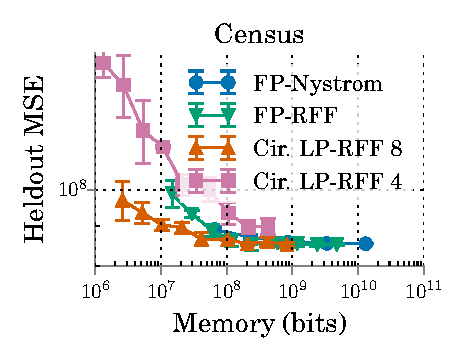
\includegraphics[width=0.3\linewidth]{figures/census_MSE_vs_n_memory.pdf} } \hfill
%		\subfigure[Census heldout MSE]{\label{fig:census_feat}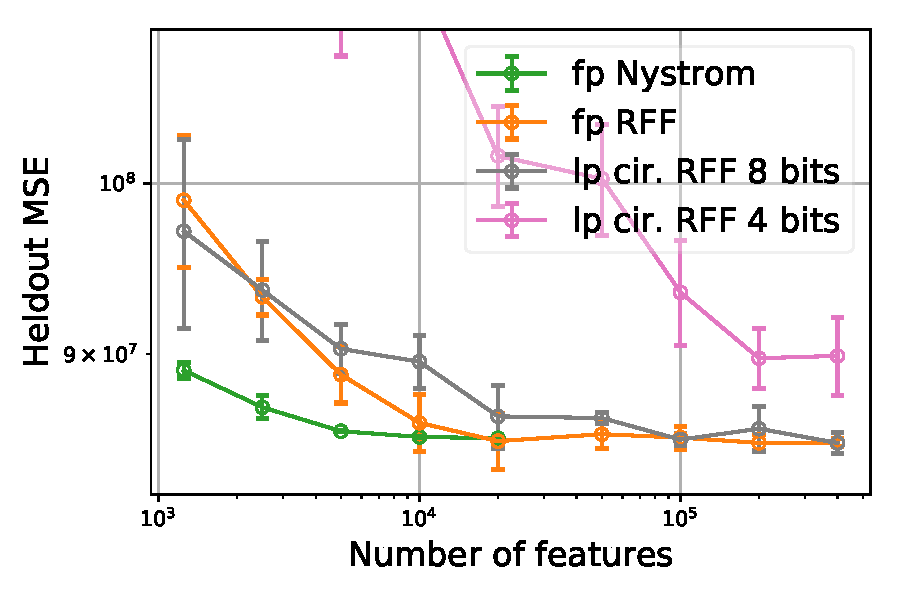
\includegraphics[width=0.3\linewidth]{figures/census_MSE_vs_n_feat.pdf} } \hfill
%		\subfigure[CovType heldout error]{\label{fig:covtype_mem} 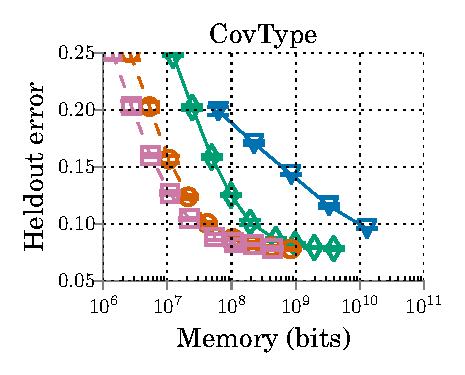
\includegraphics[width=0.3\linewidth]{figures/covtype_error_vs_n_memory.pdf} } \hfill
%		\subfigure[CovType heldout error]{\label{fig:covtype_feat}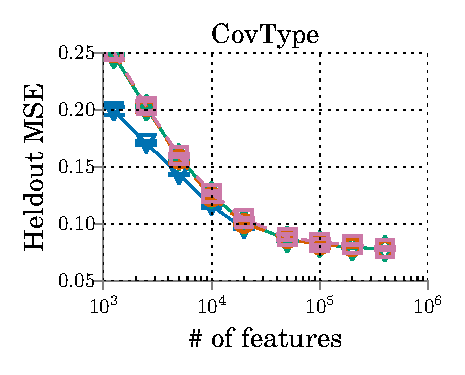
\includegraphics[width=0.3\linewidth]{figures/covtype_error_vs_n_feat.pdf} } \hfill
%		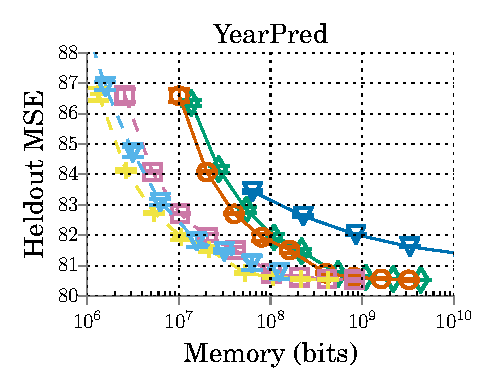
\includegraphics[width=0.3\linewidth]{figures/yearpred_MSE_vs_n_memory_all_line.pdf} &
%		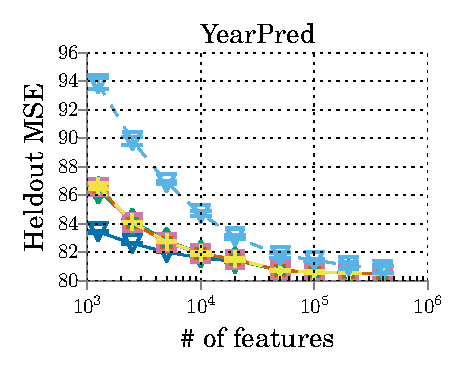
\includegraphics[width=0.3\linewidth]{figures/yearpred_MSE_vs_n_feat_all_line.pdf} &
%		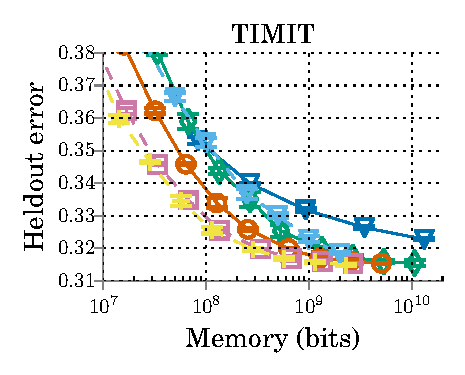
\includegraphics[width=0.3\linewidth]{figures/timit_error_vs_n_memory_all_line.pdf} &
%		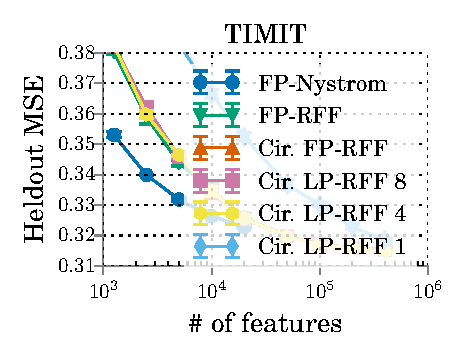
\includegraphics[width=0.3\linewidth]{figures/timit_error_vs_n_feat_all_line.pdf} \\
%		(a) Census & (b) YearPred & (c) Covtype & (d) TIMIT \\
		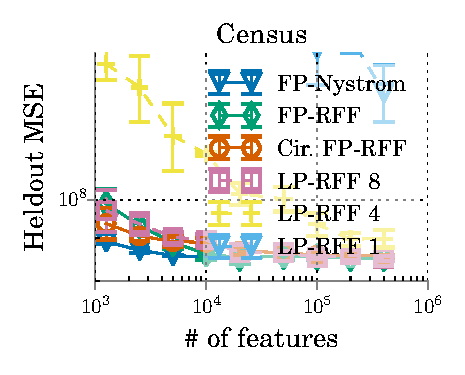
\includegraphics[width=0.4\linewidth]{figures/census_MSE_vs_n_feat_all_line.pdf} &
		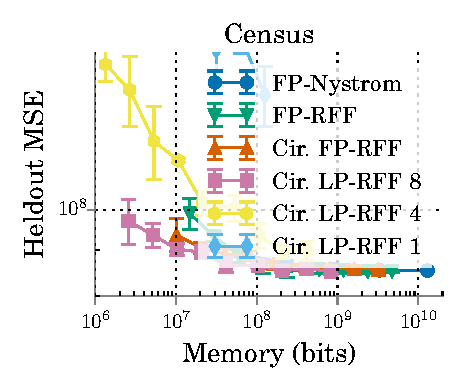
\includegraphics[width=0.4\linewidth]{figures/census_MSE_vs_n_memory_all_line.pdf} \\
		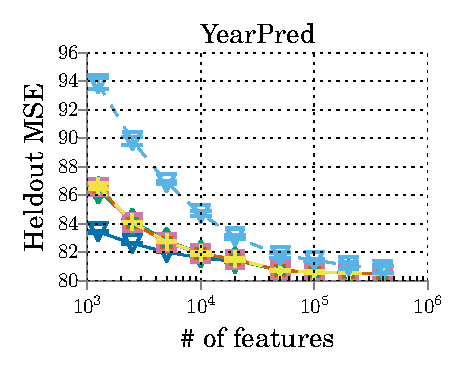
\includegraphics[width=0.4\linewidth]{figures/yearpred_MSE_vs_n_feat_all_line.pdf} &
		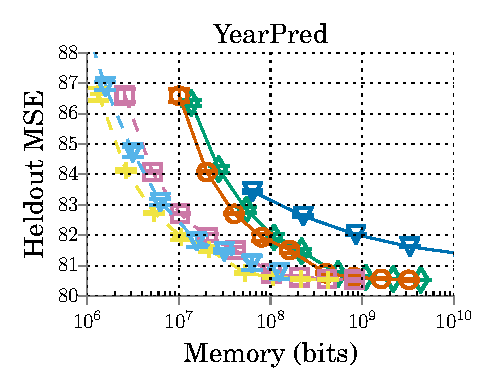
\includegraphics[width=0.4\linewidth]{figures/yearpred_MSE_vs_n_memory_all_line.pdf} \\
		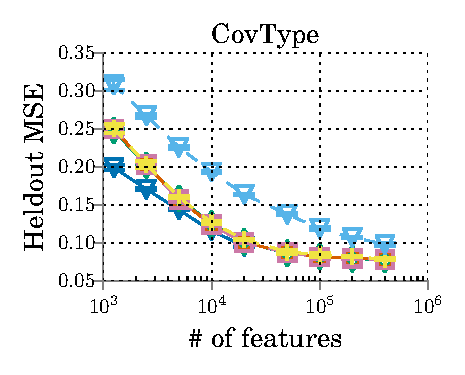
\includegraphics[width=0.4\linewidth]{figures/covtype_error_vs_n_feat_all_line.pdf} &
		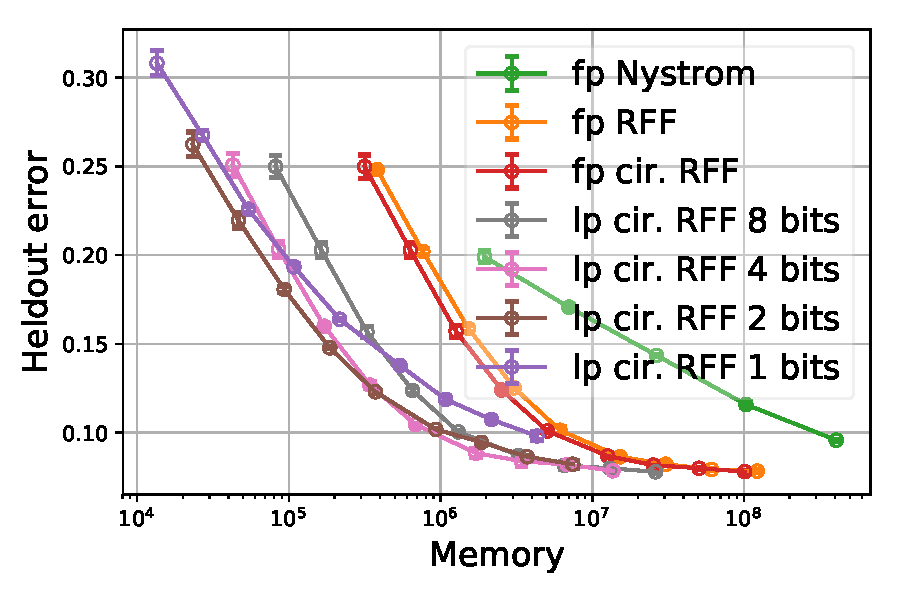
\includegraphics[width=0.4\linewidth]{figures/covtype_error_vs_n_memory_all_line.pdf} \\
		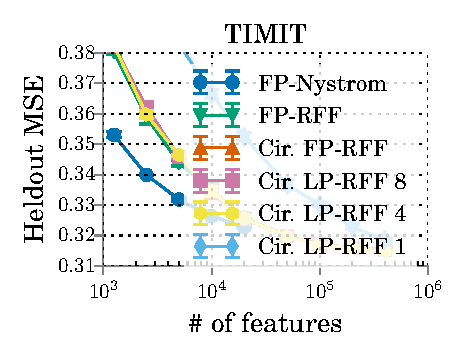
\includegraphics[width=0.4\linewidth]{figures/timit_error_vs_n_feat_all_line.pdf} &
		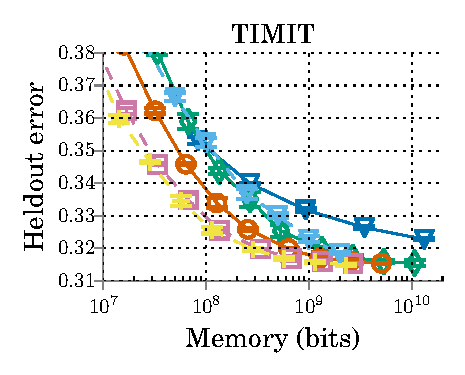
\includegraphics[width=0.4\linewidth]{figures/timit_error_vs_n_memory_all_line.pdf} \\
%		(a) Census & (b) YearPred & (c) Covtype & (d) TIMIT \\
	\end{tabular}
	\caption{Generalization performance of LP RFF, full precision RFF and \Nystrom with respect to number of features and memory budgets. We can observe that LP RFFs demonstrate better generalization performance than full precision baselines under memory budget. Noticeably, the comparison of different methods on generalization performance behaves differently under memory budget and under number off features. E.g., \Nystrom shows better generalization performance than RFF based approach with the same number of features. However, \Nystrom can be significantly worse under memory budgets.}
	\label{fig:generalization_col_app}
\end{figure}

In Section~\ref{subsec:perf_vs_rel_spec_dist}, we empirically demonstrate correlation between generalization performance and relative spectral distance. To give an extended view on the correlation, we demonstrate full results on 8, 4, 1-bits LP-RFFs, together with the full precision baselines in Figure~\ref{fig:specdist_app}. In Figure~\ref{fig:specdist_app} (left), we can observe, on both the Census and CovType datasets, relative spectral distance can be predictive for the performance across different methods; i.e. similar relative spectral distance can imply similar generalization performance across different methods. In the contrast, \Nystrom and RFF based approaches can demonstrate significantly different spectral norm and Frobenius norm of $K - \tilde{K}$, the difference of the exact kernel matrix and its approximation.

\begin{figure}
	\centering
	\begin{tabular}{@{\hskip -0.25in}c@{\hskip -0.25in}c@{\hskip -0.25in}c@{\hskip -0.25in}}
		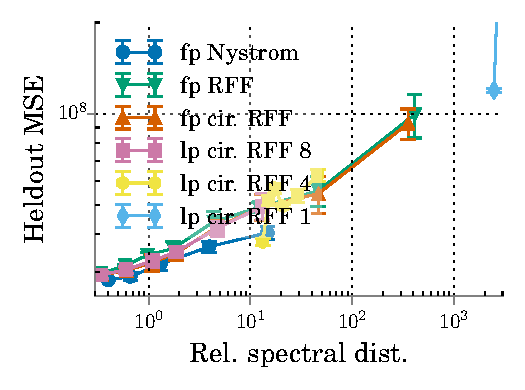
\includegraphics[width=0.33\linewidth]{figures/regression_l2_vs_delta_all_line.pdf} &
		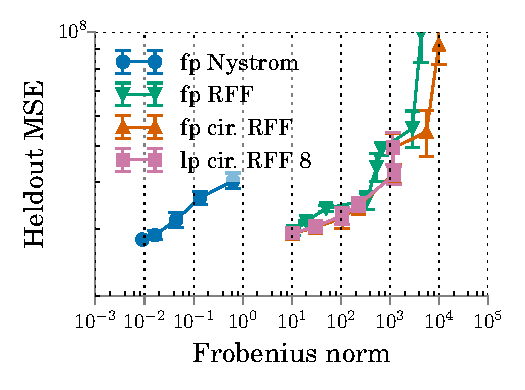
\includegraphics[width=0.33\linewidth]{figures/regression_l2_vs_f_norm_all_line.pdf} &
		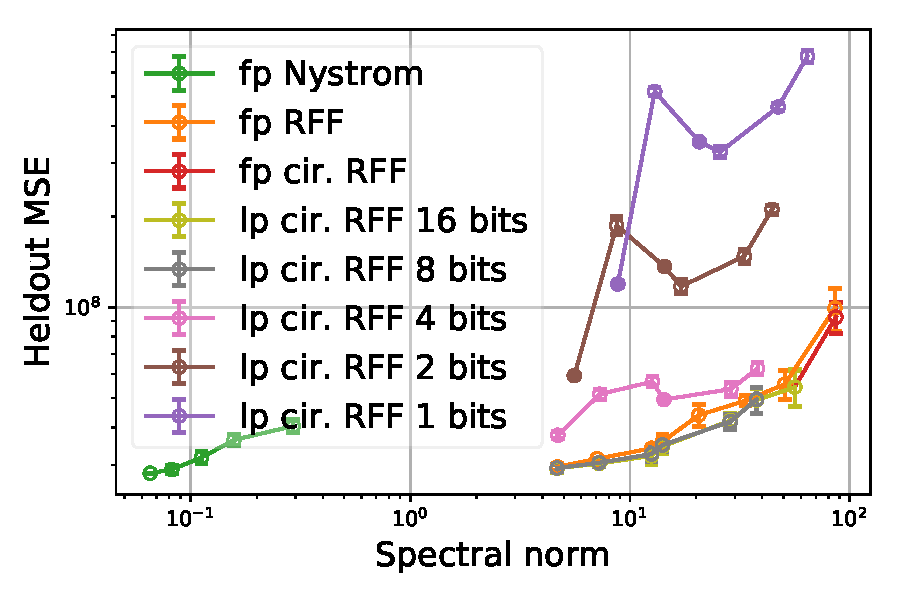
\includegraphics[width=0.33\linewidth]{figures/regression_l2_vs_s_norm_all_line.pdf} \\
		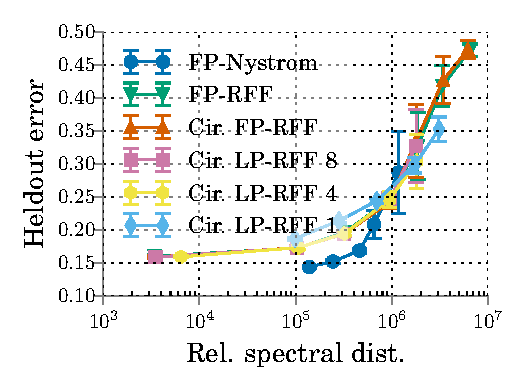
\includegraphics[width=0.33\linewidth]{figures/classification_acc_vs_delta_all_line.pdf} &
		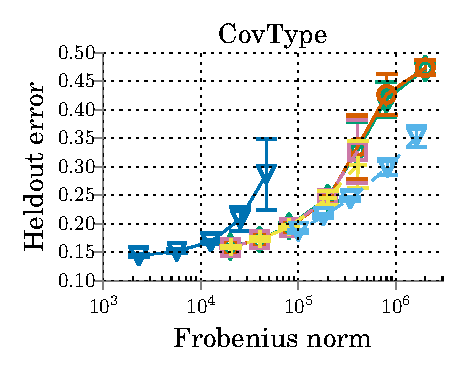
\includegraphics[width=0.33\linewidth]{figures/classification_acc_vs_f_norm_all_line.pdf} &
		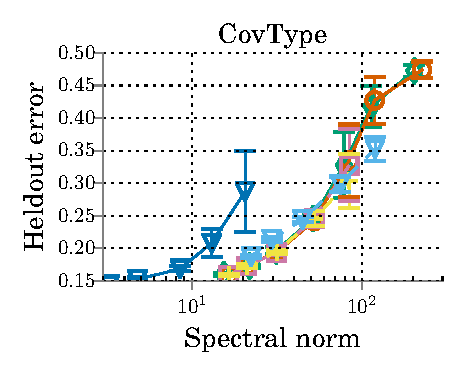
\includegraphics[width=0.33\linewidth]{figures/classification_acc_vs_s_norm_all_line.pdf} \\
	\end{tabular}
%	\begin{tabular}{@{\hskip -0.25in}c@{\hskip -0.25in}c@{\hskip -0.25in}c@{\hskip -0.25in}}
%		\subfigure[MSE and Rel. spectral distance distance]{\label{fig:census_delta_all_line} 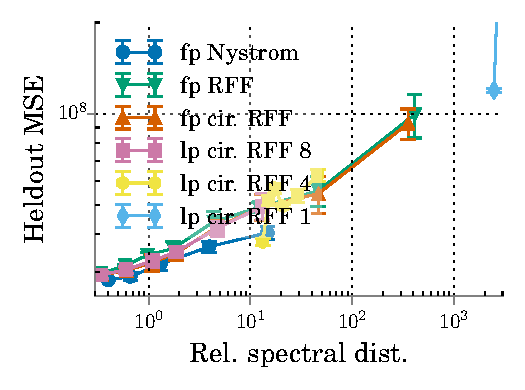
\includegraphics[width=0.33\linewidth]{figures/regression_l2_vs_delta_all_line.pdf} } \hfill
%		\subfigure[MSE and Frobenius norm]{\label{fig:census_f_norm_all_line} 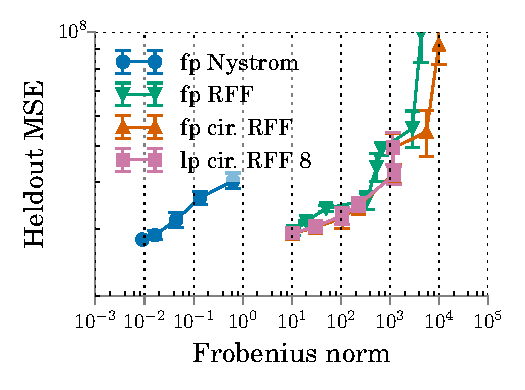
\includegraphics[width=0.33\linewidth]{figures/regression_l2_vs_f_norm_all_line.pdf} } \hfill
%		\subfigure[Rel. spectral distance distance and memory]{\label{fig:census_s_norm_all_line}  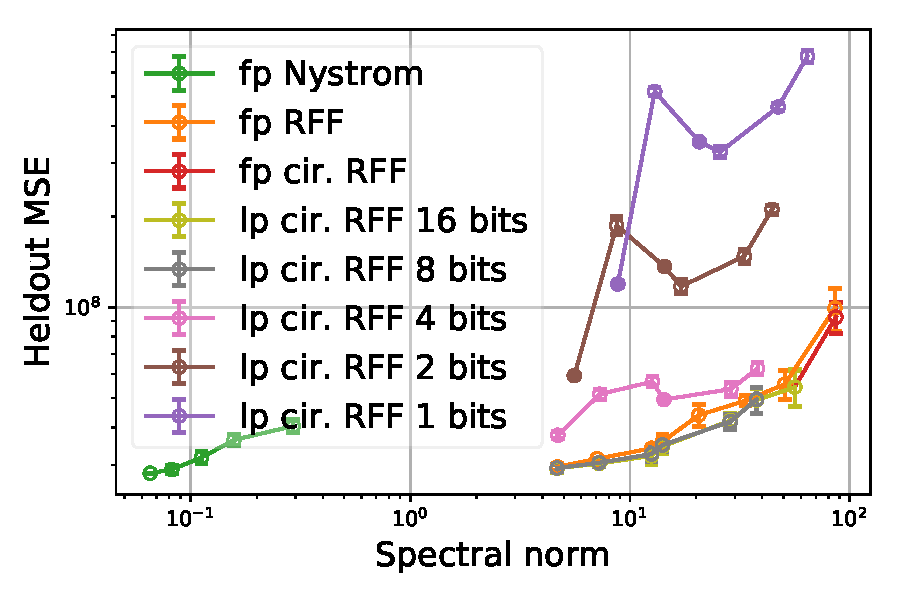
\includegraphics[width=0.33\linewidth]{figures/regression_l2_vs_s_norm_all_line.pdf} } \hfill \\
%		\subfigure[MSE and Frobenius norm]{\label{fig:covtype_delta_all_line} 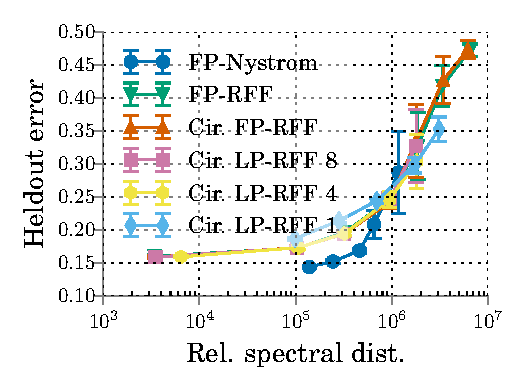
\includegraphics[width=0.33\linewidth]{figures/classification_acc_vs_delta_all_line.pdf} } \hfill
%		\subfigure[Error and Frobenius norm]{\label{fig:covtype_f_norm_all_line} 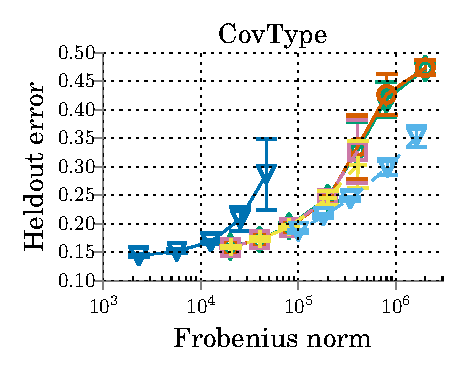
\includegraphics[width=0.33\linewidth]{figures/classification_acc_vs_f_norm_all_line.pdf} } \hfill
%		\subfigure[Error and spectral norm]{\label{fig:covtype_s_norm_all_line} 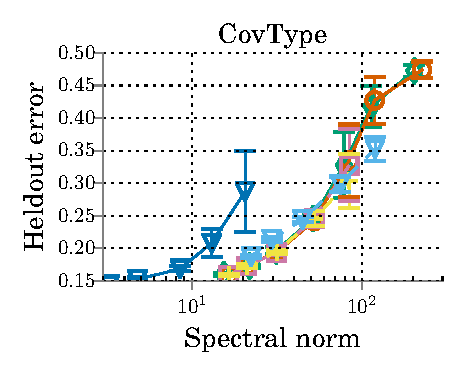
\includegraphics[width=0.33\linewidth]{figures/classification_acc_vs_s_norm_all_line.pdf}} \hfill
%	\end{tabular}
	\caption{Generalization performance vs. relative spectral distance $D_{\lambda}(K,\tK)$, and that Frobenius and spectral norms of $K - \tK$. We observe that $D_{\lambda}(K,\tK)$ aligns much better with generalization performance than the Frobenius and spectral norms, for both the Census and sub-sampled CovType datasets.}
	\label{fig:specdist_app}	
%	\begin{tabular}{c c c}
%		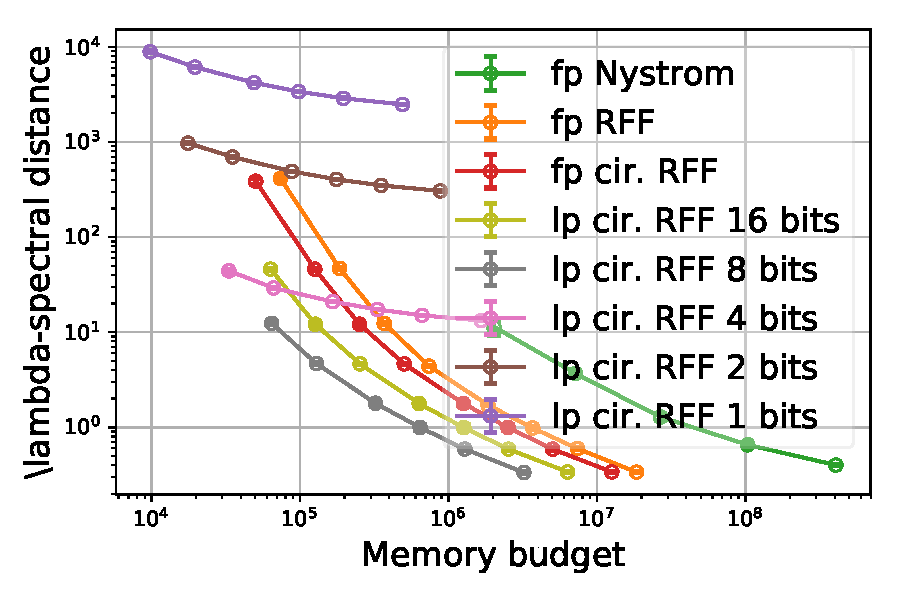
\includegraphics[width=0.33\linewidth]{figures/regression_delta_vs_mem_all_line.pdf} &
%		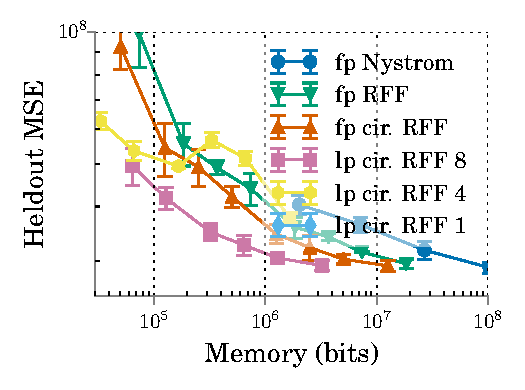
\includegraphics[width=0.33\linewidth]{figures/regression_l2_vs_mem_all_line.pdf} &
%		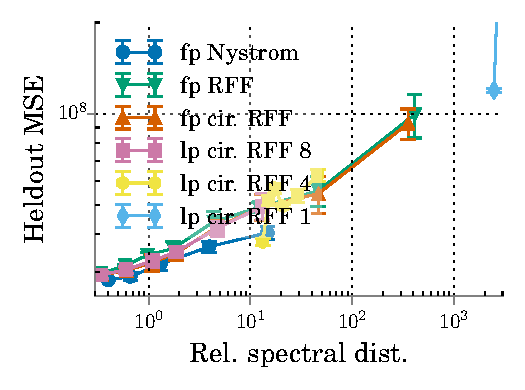
\includegraphics[width=0.33\linewidth]{figures/regression_l2_vs_delta_all_line.pdf} \\
%		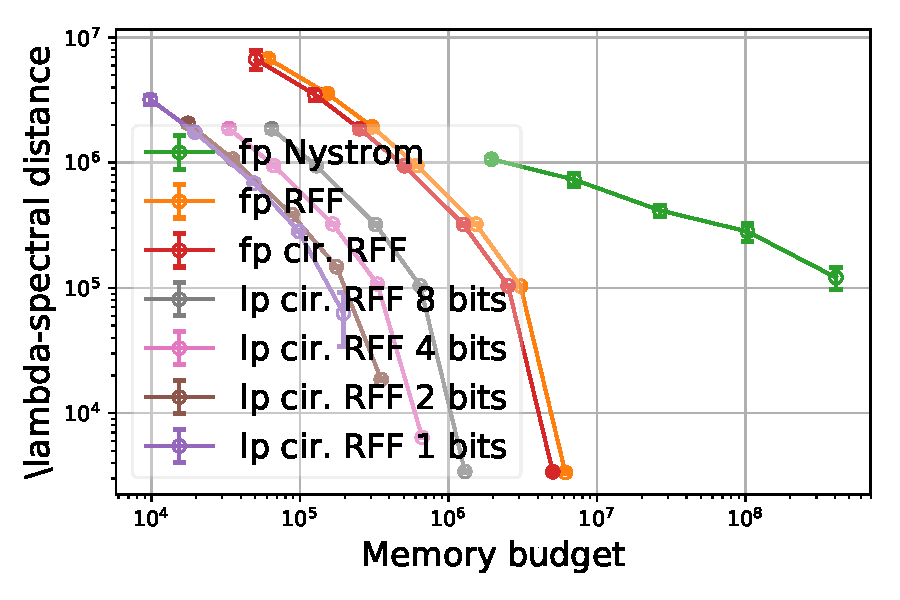
\includegraphics[width=0.33\linewidth]{figures/classification_delta_vs_mem_all_line.pdf} &
%		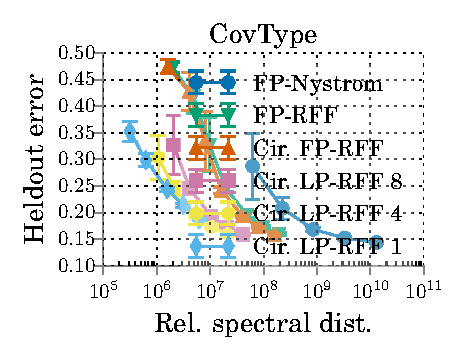
\includegraphics[width=0.33\linewidth]{figures/classification_acc_vs_mem_all_line.pdf} &
%		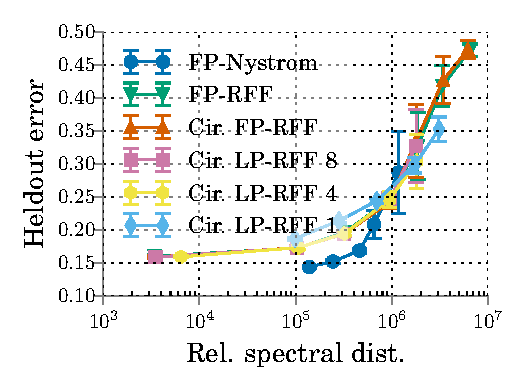
\includegraphics[width=0.33\linewidth]{figures/classification_acc_vs_delta_all_line.pdf} \\
%		(a) & (b) & (c)
%	\end{tabular}
%	\caption{The strong correlation between generalization performance and $\lambda$-spectral distance $D_{\lambda}(K,\tK)$ under memory budgets for the Census dataset (top) and subsampled CovType dataset (bottom). Under different memory budget in (a) and (b), the precision demonstrates smaller $D_{\lambda}(K,\tK)$ tends to have better generalization performance. In (c), different kernel approximation approaches demonstrate similar generalization performance for similar $\lambda$-spectral distance.}
%	\label{fig:specdist_app}
\end{figure}

